\chapter{Experimentos e Resultados}
\label{ch:07}

Este capítulo será dedicado a explanações sobre o modelo construído e às predições resultantes. A Seção \ref{sec:treinamento} de treinamento do modelo trata especificamente dos hiperparâmetros\footnote{colocar alguma coisa aqui} utilizados e dos resultados das métricas utilizadas. Após o treinamento do modelo, segue a etapa de decodificação dos outputs (citada no Capítulo \ref{ch:05}). Somente nesta etapa pode-se analisar os verbos preditos pela rede e avaliar a acurácia obtida pelo modelo. A Seção \ref{sec:results} introduz a metodologia utilizada para a avaliação dos resultados das decodificações e apresenta uma visão geral do desempenho do modelo para cada classe de verbo. Em seguida, a Seção \ref{sec:interesting} analisa com mais detalhes resultados interessantes obtidos pelo modelo. 

\section{Treinamento}
\label{sec:treinamento}

Como foi introduzido no Capítulo \ref{ch:03}, o treinamento do modelo de redes neurais consiste sempre na introdução de um input em paralelo com seu alvo correspondente. Ficou faltando, porém, uma discussão de cunho prático a respeito da frequência em que esses dados são apresentados ao modelo. Essa discussão é importante pois a frequência é um dos fatores mais relevantes para o ajuste dos pesos das redes. Uma frequência muito baixa não é o suficiente para causar grandes modificações nos pesos, fenômeno conhecido como \textit{underfit}. Em contrapartida, uma frequência muito alta faz com que o modelo se torne especialista nos dados de treinamento, porém se torna incapaz de lidar com dados nunca antes vistos, fenômeno conhecido como \textit{overfit}. Para encontrar a frequência ideal, utiliza-se como auxílio um gráfico conhecido como curva de aprendizado, como o apresentado na Figura \ref{fig:training2000}. No ramo da modelagem em redes neurais, cada vez que o grupo de dados de treino é introduzido completamente no modelo, configura-se o que é chamado de uma \textit{época}. Ainda, no caso do corpus em questão, optou-se pela realização do treinamento sem repetições de verbos por época.  

Nos três primeiros gráficos da figura, exibem-se três diferentes métricas de avaliação em relação ao número de épocas realizadas. 
Como se pode observar, a partir de aproximadamente 300 épocas, a curva de aprendizado começa a se estabilizar em torno de um valor. Também é possível ver a diferença entre os scores de treino (curva azul) e teste (curva laranja). Essa diferença mostra que os dados de treino não estão sendo suficientes para aumentar o score nos dados de teste. Desse modo, concluiu-se que 300 épocas seria o momento de conclusão do treinamento do modelo. Os resultados nessa nova escala podem ser observados na Figura \ref{fig:training}.  

\begin{figure}[H]
  \centering
  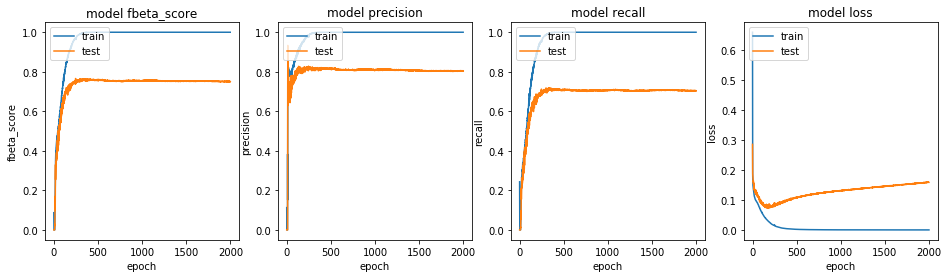
\includegraphics[width=1.0\linewidth]{img/2000_precision.png}
  \caption{Curva de Aprendizado para 2000 épocas}
  \label{fig:training2000}
\end{figure}

\begin{figure}[H]
  \centering
  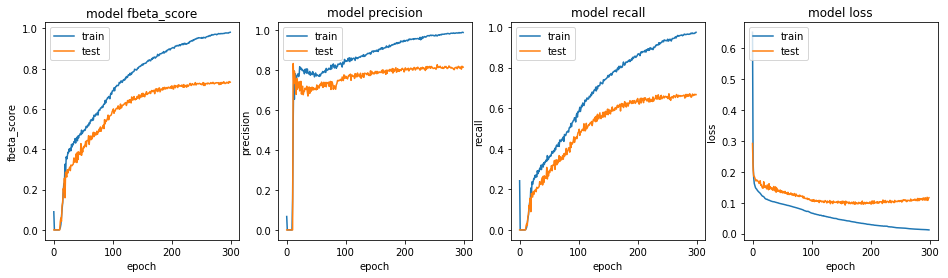
\includegraphics[width=1.0\linewidth]{img/300_fbeta.png}
  \caption{Curva de apredizado para 300 épocas}
  \label{fig:training}
\end{figure}

Para o entendimento das métricas utilizadas, faz-se necessária uma recapitulação a respeito do que se espera como output do modelo. Para cada verbo, o modelo prediz uma sequência de $n$ vetores de tamanho 21 (o número total de traços fonéticos somado ao tokens de início e final), aonde $n$ é o número de fones do verbo alvo e cada vetor corresponde a um fone. Esses 21 valores são arredondados para 0 ou 1 dependendo de um determinado limiar, que neste caso é 0.5. As métricas são calculadas comparando-se esses $n$ vetores de output com seus respectivos alvos.

A precisão é uma métrica calculada de acordo com a Equação \ref{eq:precision}. Nesta métrica, avalia-se a proporção de verdadeiros positivos ($vp$) em relação ao número total de positivos que o modelo previu, ou seja, dentre os traços fonéticos preditos pelo modelo, quantos estavam de acordo com os presentes no alvo.


\begin{align}\label{eq:precision}
\text{Precisão = } \frac{vp}{vp + fp}
\end{align}

O \textit{Recall}, também conhecido como revocação, foi calculado a partir da Equação \ref{eq:recall}. Nesta métrica busca-se entender a proporção de traços fonéticos que o modelo previu (verdadeiros positivos) em relação a todos que ele deveria ter previsto (verdadeiros positivos + falsos negativos). 

\begin{align}\label{eq:recall}
\text{Recall = } \frac{vp}{vp + fn}
\end{align}

Por fim, o F1 Score (Eq. \ref{eq:f1}) é a média harmônica das duas métricas já explanadas.

\begin{center}
\begin{align}\label{eq:f1}
  \text{F1 Score} = 2 \times \frac{precision \times recall}{precision + recall}
  \end{align}
\end{center}

Todas as métricas variam no intervalo [0,1] sendo que valores próximos a 1 indicam alto desempenho do modelo.
Os resultados exibidos na Figura \ref{fig:training} mostram que a métrica Recall atinge scores mais baixos que a precisão. Isso significa que o modelo tem uma certa tendência a gerar outputs com mais valores nulos do que deveria. A Precisão atingiu valores próximos a 0.8. Isso indica que o modelo prevê aproximadamente 20\% dos traços de forma equivocada.

O último gráfico da figura é o gráfico do Erro, já explanado no Capítulo \ref{ch:03}. Em uma situação ideal a curva de erro do teste deve tender a zero, porém vê-se que o erro apresenta um comportamento de queda até em torno de 100 épocas e depois começa a subir gradualmente. 



\section{Resultados da Decodificação}
\label{sec:results}
Como o tamanho do corpus disponível é limitado, não é interessante realizar um único experimento com uma única segmentação entre treino e teste, pois haveriam verbos em que o modelo nunca seria testado e outros que nunca seriam utilizados no treinamento. Dessa forma a acurácia do modelo poderia variar bastante dependendo dos verbos sorteados para cada um desses grupos. Assim, uma técnica de validação cruzada chamada \textit{K-Fold} (indicar referencia) foi escolhida para o estudo dos resultados. A análise K-Fold permite que o modelo seja avaliado em todos os verbos do corpus. A técnica consiste, primeiramente, na formação de K subconjuntos de verbos mutuamente exclusivos de tamanhos próximos (idênticos caso a divisão por K seja exata). Em seguida, um desses subconjuntos é escolhido como o conjunto de teste enquanto que os K-1 restantes são utilizados como treino. O tamanho de K é definido a partir da escolha de proporção em que se deseja realizar a segmentação entre treino e teste, ou seja, para sempre manter a proporção de testes em 20\% de modo que estes verbos sejam sempre diferentes, o corpus precisa ser segmentado em 5 subconjuntos distintos. O desenho \ref{fig:kfold} ilustra o algoritmo. 

\definecolor{blue}{RGB}{159, 192, 176}
\definecolor{green}{RGB}{160, 227, 127}
\definecolor{orange}{RGB}{243, 188, 125}
\definecolor{red}{RGB}{253, 123, 84}
\definecolor{nephritis}{RGB}{39, 174, 96}
\definecolor{emerald}{RGB}{46, 204, 113}
\definecolor{turquoise}{RGB}{39, 174, 96}
\definecolor{green-sea}{RGB}{22, 160, 133}
\definecolor{purple}{RGB}{181, 124, 215}
% Tikzstyles for Computation Graphs

% nodes
\tikzstyle{noop} = [circle, draw=none, fill=red, minimum size = 10pt]
\tikzstyle{op} = [circle, draw=red, line width=1.5pt, fill=red!70, text=black, text centered, font=\bf \normalsize, minimum size = 25pt]

\tikzstyle{opintense} = [circle, draw=red, line width=1.5pt, fill=red!150, text=black, text centered, font=\bf \normalsize, minimum size = 25pt]


%new style
\tikzstyle{gp} = [circle, draw=red, line width=4pt, text=black, text centered, font=\bf \normalsize, minimum size = 4.cm]

\tikzstyle{box} = [rectangle, draw=red, line width=1.5pt, fill=red!70, text=black, align=center, font=\bf \normalsize, minimum size = 45pt]

\tikzstyle{box2} = [rectangle, draw=black, line width=0.9pt, text=black, align=center, font=\bf \normalsize, minimum size = 20pt]

\tikzstyle{box3} = [rectangle, draw=black, line width=0.9pt, fill=black, text=black, align=center, font=\bf \normalsize, minimum size = 20pt]

\tikzstyle{state} = [circle, draw=blue, line width=1.5pt, fill=blue!70, text=black, text centered, font=\bf \normalsize, minimum size = 25pt]

\tikzstyle{output} = [circle, draw=purple, line width=1.5pt, fill=purple!70, text=black, text centered, font=\bf \normalsize, minimum size = 25pt]


\tikzstyle{gradient} = [circle, draw=nephritis, line width=1.5pt, fill=nephritis!60, text=black, text centered, font=\bf \normalsize, minimum size = 25pt]
\tikzstyle{textonly} = [draw=none, fill=none, text centered, font=\bf \normalsize]
\tikzstyle{boxtextonly} = [draw=none, fill=none, align=center, font=\bf \normalsize]

\tikzstyle{normal} = [circle, draw=black, line width=1.0pt, fill=none, text=black, text centered, font=\bf \normalsize, minimum size = 20pt]


% edges
\tikzstyle{tedge}  = [draw, thick, >=latex, ->]
\tikzstyle{tedge_dashed}  = [draw, thick, >=latex, ->, dashed]
\tikzstyle{nedge}  = [draw, thick, >=latex]
\tikzstyle{nedge_dashed}  = [draw, thick, >=latex, dashed]


% namedscope
\tikzstyle{namedscope} = [circle, draw=orange, line width=1.5pt, fill=orange!60, align=center, inner sep=0pt]
\begin{figure}[ht!]
\centering

\scalebox{1.0}{
\begin{tikzpicture}[H]

%first
\node[box3] (box1) {};
\node[box2, right=0pt of box1] (box2) {};
\node[box2, right=0pt of box2] (box3) {};
\node[box2, right=0pt of box3] (box4) {};
\node[box2, right=0pt of box4] (box5);

%second
\node[box2, below=15pt of box1] (box6) {};
\node[box3, right=0pt of box6] (box7) {};
\node[box2, right=0pt of box7] (box8) {};
\node[box2, right=0pt of box8] (box9) {};
\node[box2, right=0pt of box9] (box10);

%third
\node[box2, below=15pt of box6] (box11) {};
\node[box2, right=0pt of box11] (box12) {};
\node[box3, right=0pt of box12] (box13) {};
\node[box2, right=0pt of box13] (box14) {};
\node[box2, right=0pt of box14] (box15);

%fourth
\node[box2, below=15pt of box11] (box16) {};
\node[box2, right=0pt of box16] (box17) {};
\node[box2, right=0pt of box17] (box18) {};
\node[box3, right=0pt of box18] (box19) {};
\node[box2, right=0pt of box19] (box20);

%fifth
\node[box2, below=15pt of box16] (box21) {};
\node[box2, right=0pt of box21] (box22) {};
\node[box2, right=0pt of box22] (box23) {};
\node[box2, right=0pt of box23] (box24) {};
\node[box3, right=0pt of box24] (box25);

%legenda
\node[box2, right=35pt of box10] (box26) {};
\node[textonly, right=5pt of box26] (box27) {Treino};
\node[box3, below=10pt of box26] (box28) {};
\node[textonly, right=5pt of box28] (box29) {Teste};



\end{tikzpicture}
}\caption{Técnica de segmentação do Corpus via K-Fold} 
\label{fig:kfold}
\end{figure}

Além disso, há ainda a vantagem do algoritmo de estratificação, ou seja, a possibilidade de que, em cada um dos treinamentos, as proporções das classes de verbos se mantenham no treinamento. Isso significa que, por exemplo, a classe de irregularidades 12 (testar -> tEstu) que possui 20 verbos, terá sempre 16 verbos verbos no treinamento e 4 no teste. Assim, após os 5 treinamentos diferentes, todos os verbos da classe foram testados e há a certeza de que haviam verbos dessa classe no treinamento. 

Ainda, como há um fator de aleatoriedade devido às inicializações dos pesos e também como os itens de treino e teste são sorteados pelo algoritmo no momento da segmentação do K-Fold, os resultados da rede podem variar. Para uma melhor compreensão de como ocorre essa variação para cada classe, foram realizadas 30 análises K-Fold. As acurácias e seus respectivos desvios são exibidos nas subseções a seguir. Nestas, também busca-se encontrar possíveis fatores que tenham influenciado nos resultados obtidos.
%Dentre esses experimentos, a acurácia mais alta obtida foi de 17\% (73 verbos). As análises a seguir foram feitas no intuito de se entender melhor as situações de maior dificuldade do modelo.

\subsection{A relação entre acurácia e a proporção da classe no corpus}
\label{sec:prop}
Um fator que pode influenciar no resultado é o tamanho do corpus e o desbalanceamento das classes. Portanto, cabe verificar se há alguma relação entre a proporção da classe no corpus e a acurácia. Na Fig.\ref{fig:kfoldprop} é possível observar que as acurácias de algumas das classes de verbos seguem uma certa tendência linear de acordo com as suas respectivas proporções no corpus, enquanto que há um outro grupo de classes que apresenta acurácia mais baixa independentemente da proporção. O coeficiente de correlação de Pearson encontrado entre essas variáveis foi de 0.42.

\begin{figure}[H]
  \centering
  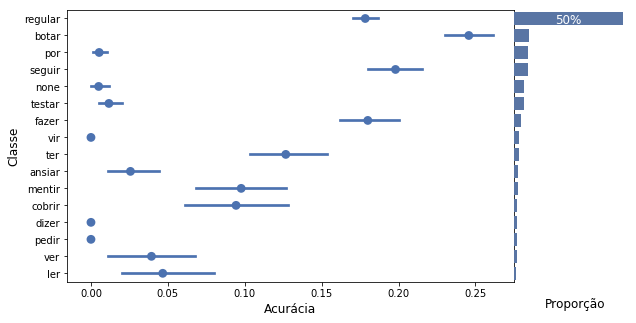
\includegraphics[width=0.8\linewidth]{img/proporxacc.png}
  \caption{Acurácia Ordenada pela Proporção das Classes}
  \label{fig:kfoldprop}
\end{figure}

Para entender os resultados obtidos, o experimento com a acurácia mais alta (vide apêndice) será utilizado como referência para a análise de erros.

Ao analisar os erros ocorridos na classe do verbo “Pôr“, verifica-se que praticamente um terço (8/26) dos erros cometidos foram erros de \textit{regularização}, ou seja, o modelo se confundiu com a classe mais presente (a classe dos verbos regulares) e manteve o padrão de flexão regular. Em seguida, a próxima classe com acurácia baixa fora da tendência é a classe de verbos sem classe. Esse resultado era totalmente esperado pois não havia outros verbos no corpus para que o modelo conseguisse detectar possíveis padrões para fazer predições corretas. A classe do verbo “testar” apresentou muitas predições incoerentes, porém também houve erros de regularização (4/19). Ainda sobre essa classe, chama a atenção que para o verbo “pegar“, o modelo acertou a flexão irregular transformando a vogal anterior meio-fechada em meio-aberta, porém por algum motivo ficou faltando o traço de vozeamento para caracterizar o fone “g” ao invés de “k”, o que resultou na flexão equivocada de pegar $\rightarrow$ pEku. A classe do verbo “vir”, por sua vez, apresentou 5/11 de erros por regularização, os demais parecem erros bastante incoerentes. A classe do verbo “ansiar” também parece estar fora da tendência, apresentou 7 erros incoerentes e quase acertou a flexão do verbo “passear“, porém substituiu a consoante “s” por “r“, ambas alveolares. Por fim, a classe do verbo “dizer” apresentou apenas erros incoerentes e a classe do verbo “pedir” acertou a flexão irregular no verbo “pedir” porém não transformou o fone “d” em “s” (alveolar - surda - fricativa). Ao invés disso, previu “t” (alveolar - surda - oclusiva). Novamente, errou por causa de apenas de um traço fonético.

Os erros observados motivaram o estudo de outras variáveis em relação a acurácia. Não obstante, a métrica de acurácia parece inadequada visto que em muitos casos o modelo foi capaz de identificar a flexão apropriada, porém se confundiu em um único traço distintivo, como no caso do verbo “pega”.



\subsection{A relação entre acurácia e a perplexidade de cada classe}

Outra variável que poderia influenciar nos resultados seria uma maior variabilidade, ou imprevisibilidade, de algumas classes em relação a outras. Suponha que exista uma classe na qual todos os verbos compartilhem do mesmo comprimento e variações mínimas, por exemplo:

\begin{center}
    akabar - abalar - akalar - asolar
\end{center}

Essa classe, por conter pouca variabilidade de fones, poderia ter vantagem em relação a uma outra em que há maior variabilidade, como por exemplo:

\begin{center}
    dezenkontrar - estourar - akal3ntar - sust3ntar - axar
\end{center}

Para quantificar as previsibilidades das classes, foi utilizada a medida de perplexidade. Em teoria da informação (ref), a perplexidade é uma medida do quão bem um modelo de probabilidade prevê uma amostra. Por esse motivo ela é bastante utilizada como referência para a comparação entre diferentes modelos de linguagem. Uma baixa perplexidade indica que o modelo proposto é bom em prever a amostra. O gráfico na Figura \ref{fig:kfoldperp} mostra a relação entre a acurácia do modelo e a perplexidade das classes, obtida a partir de um modelo de trigramas.  %A equação (tal) exibe a fórmula para o cálculo da métrica.


\begin{figure}[H]
  \centering
  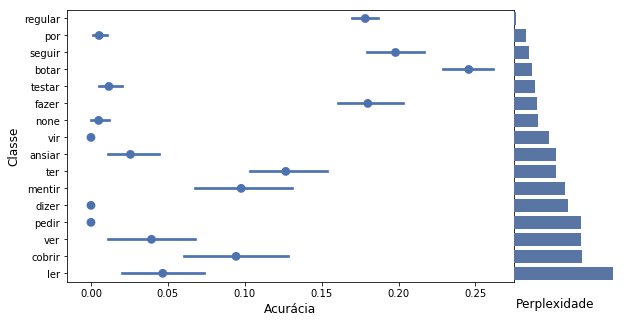
\includegraphics[width=0.8\linewidth]{img/perplexidade.png}
  \caption{Acurácia por Perplexidade}
  \label{fig:kfoldperp}
\end{figure}

Nota-se que a relação entre as duas variáveis é menos clara, com um coeficiente de correlação de Pearson = 0.38. 

\subsection{A relação entre acurácia e o comprimento médio dos verbos de cada classe}

Outra questão que poderia influenciar na performance do modelo é o número médio de fones dos verbos na classe.  O verbo “3ntret3Nu” (entretenho), por exemplo, contém 9 fones para serem preditos. Como cada fone contém 21 traços, no total o modelo tem que conseguir prever 189 números. O verbo “falu” (falo), em contrapartida, possui 4 fones, ou seja, 84 números a serem preditos. Dessa forma, é natural pensar que quanto maior o número de predições necessárias, maior a possibilidade do modelo cometer algum erro. Apesar disso, a Figura \ref{fig:kfoldprop} não mostra uma relação nítida entre a acurácia e o comprimento médio com uma correlação de Pearson = 0.39.

\begin{figure}[H]
  \centering
  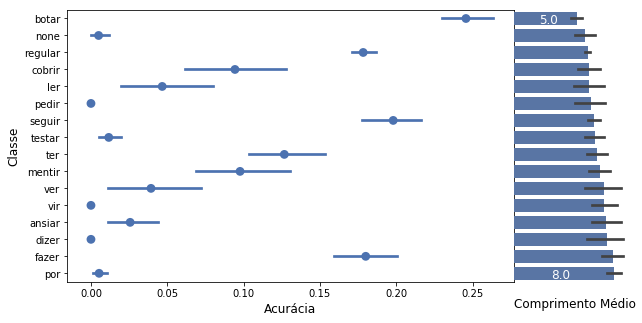
\includegraphics[width=0.8\linewidth]{img/comp_acc.png}
  \caption{Acurácia por Comprimento Médio}
  \label{fig:kfoldprop}
\end{figure}


% colocar no apendice os resultados
\section{Resultados e Erros Relevantes}
\label{sec:interesting}

Alguns erros interessantes como troca de classes e regularizações já foram apresentados na Seção \ref{sec:prop}, mas ainda há outros erros que merecem destaque. (Ver Apêndice para tabela completa com Classe, Input, Output e Alvo)

Na classe dos verbos sem agrupamento, um erro notável foi a flexão realizada para o verbo trazer (“trasu”), o que mostra que o modelo identificou o padrão de flexão da classe do verbo “fazer”. 

Na classe do verbo “pedir”, apresentou a flexão “espidu” para o verbo “espedir”, o que denota uma possível confusão com a classe do verbo “conseguir”.

Nos verbos regulares nota-se a presença de vários erros devido a troca de apenas um traço fonético. Como por exemplo para o verbo “convidar”, o output resultante foi “konviru”. Para o verbo “convencer”, “konfensu”.

Para os verbos da classe do verbo “seguir“, três verbos foram flexionados de acordo com a família do verbo “testar“. São eles: “ferir” (fEru), “vestir” (vEstu) e “repetir” (hepEtu).

A classe do verbo “ver” também apresentou erros interessantes: a confusão com a classe do verbo “vir” nos verbos “prever” (“preveNu”) e “entrever” (“entreveNu”). Também por pouco não acertou o alvo no verbo “rever” (hefexu), ficou faltando o traço de vozeamento nas duas últimas consoantes.
